We, now,  evaluate how $\varepsilon_{\winlen}$ varies with $\sigma_\dpintvl$, $\varnumupdates$, and $\ssens$.
All analyses use $\delta_\winlen = 10^{-6}$.
We consider two different classes of applications based on their sensitivity ($qsens$): applications with high sensitivity such as video streaming and applications with lower value of sensitivity such as web browsing.
The sensitivity value represents the highest potential change in the buffering queue size when two distinct traffic traces pass through the shaping mechanism.
% If the change in queue size surpasses the sensitivity value, it results in a privacy loss exceeding the intended $\varepsilon_{\winlen}$ threshold.
% Nevertheless, the privacy guarantees provided by Differential Privacy (DP) remain applicable even in cases where the privacy loss exceeds the sensitivity, resulting in traffic shaping with larger privacy loss values.


\Cref{subfig:high-sensitivity-epsilon-sigma} and \Cref{subfig:low-sensitivity-epsilon-sigma} show the trade-off between privacy loss ($\varepsilon_{\winlen}$) and noise ($\sigma_\dpintvl$) over four different numbers of DP measurements ($\varnumupdates$) for two different setups.
Intuitively, a larger $\sigma_\dpintvl$ implies higher bandwidth overhead due to DP shaping.
Besides that, applications with higher sensitivity, denoted as $\ssens$, particularly require larger values of $\sigma_\dpintvl$ to provide the same levels of privacy guarantees.
For example, for an application with a sensitivity of $\varepsilon_{\winlen}=1MB$, according to \Cref{subfig:low-sensitivity-epsilon-sigma}, to retain a total privacy loss $\varepsilon_{\winlen} = 1$ with at most 4 DP measurements, we need to add noise with $\sigma_\dpintvl = 6 MB$ for each DP measurement.
Meanwhile, to have the same value of privacy loss with 4 DP measurement in an application with a lower sensitivity $\varepsilon_{\winlen}$, we need to add noise with $\sigma_\dpintvl = 0.8 MB$.

The large gap between theoretical privacy guarantees and the effectiveness of the state-of-the-art attacks, as discussed in \Cref{sec:eval-empirical-privacy}, is also noteworthy in this context.
For example, $\varepsilon_{\winlen} = 100$ with 4 DP measurements (the approximate configuration that defeats the classifiers in \Cref{fig:empirical-privacy}) only requires $\sigma_\dpintvl < 0.1 MB$ even for high-sensitivity applications.
However, we configure our system to provide theoretical guarantees (\ie small values of privacy loss), and discuss how to amortize bandwidth overheads using concurrent flows without increasing privacy loss in \Cref{sec:eval-bw}.

Using these plots, an application can choose suitable values of $\ssens$ and $\winlen$ to determine the trade-off between $\varepsilon_{\winlen}$ and $\delta_{\winlen}$.
For our web application serving static HTML, we recommend $\winlen = 1s$, since web page downloads in our AWS setup finished within 1s, and $\ssens = 150 KB$, which covers 95\% of the web pages in our dataset.
Similarly, In \Cref{fig:empirical-privacy}, we explain the choices for our video application.
Using $\varepsilon_{\winlen}$ and $\dpintvl$, we can further determine the aggregate privacy loss over longer traffic streams using R\'enyi-DP composition.
For instance, with $\varepsilon_{\winlen} = 1$, $\winlen = 5s$, and $\dpintvl = 1s$, the total privacy loss for a 5 min video, which generates 300 DP measurements at 1s intervals, is 8.92; the total loss for a 1 hr video is 38.8.
We emphasize that {\em $\ssens$ and $\varepsilon_\winlen$ should be selected using trade-off plots similar to \Cref{fig:privacy-microbenchmarks-high-sensitivity} and \Cref{fig:privacy-microbenchmarks-low-sensitivity} independently of the application's dataset.}
Another approach to parameter configuration within our setup involves utilizing a publicly available dataset for the same application, such as a publicly accessible video streaming dataset or web service dataset.
This allows for the independent configuration of parameters, which can then be deployed within our system, irrespective of users' traffic. This approach, however, requires a measurement study to find proper parameters for different applications. We discuss this in \Cref{sec:conclusion-future}.


\begin{figure}[t]
  \centering
  \begin{subfigure}{0.49\columnwidth}
      \centering
      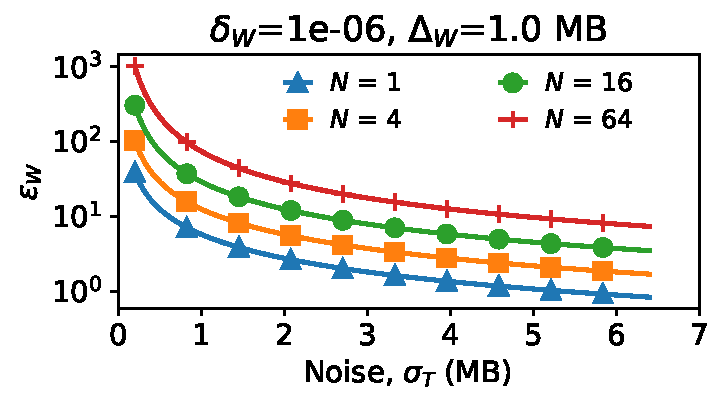
\includegraphics[width=\textwidth]{plots/privacy_loss_VS_noise_std_video.pdf}
      \caption{}
      %        \caption{Noise vs privacy loss}
      \label{subfig:high-sensitivity-epsilon-sigma}
  \end{subfigure}
  \hfill
%    \begin{subfigure}{0.33\textwidth}
  %        \centering
  %
  %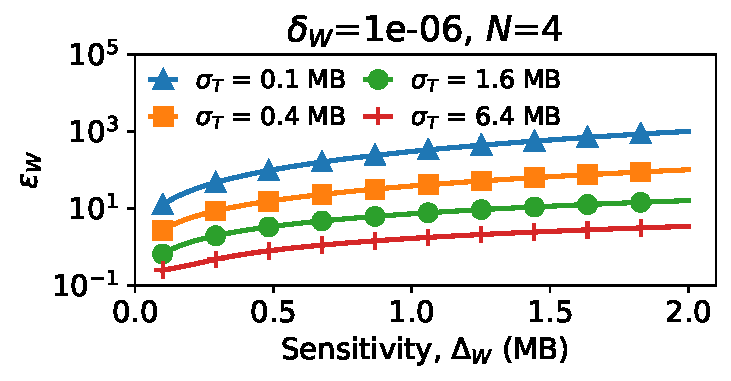
\includegraphics[width=\textwidth]{plots/privacy_loss_VS_sensitivity_video.pdf}
  %        \caption{Sensitivity vs privacy loss}
  %        \label{subfig:high-sensitivity-epsilon-sensitivity}
  %    \end{subfigure}
%    \hfill
  \begin{subfigure}{0.49\columnwidth}
      \centering
      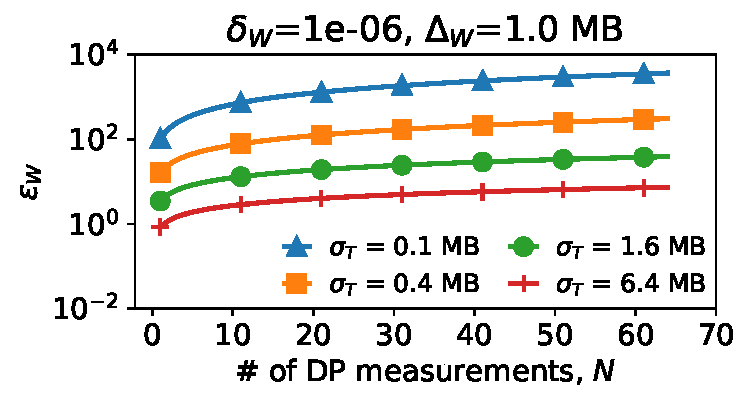
\includegraphics[width=\textwidth]{plots/privacy_loss_VS_query_num_video.pdf}
      \caption{}
%        \caption{\# of DP measurements vs privacy loss}
      \label{subfig:high-sensitivity-epsilon-queries}
  \end{subfigure}
  \caption{
    Per-window privacy loss ($\varepsilon_{\winlen}$) as a function of
    (a) noise ($\sigma_\dpintvl$), and (b) number of DP measurements ($N$).
%    \am{Make notations consistent.}
  }
  \label{fig:privacy-microbenchmarks-high-sensitivity}
\end{figure}


\begin{figure}[t]
  \centering
  \begin{subfigure}{0.49\columnwidth}
      \centering
      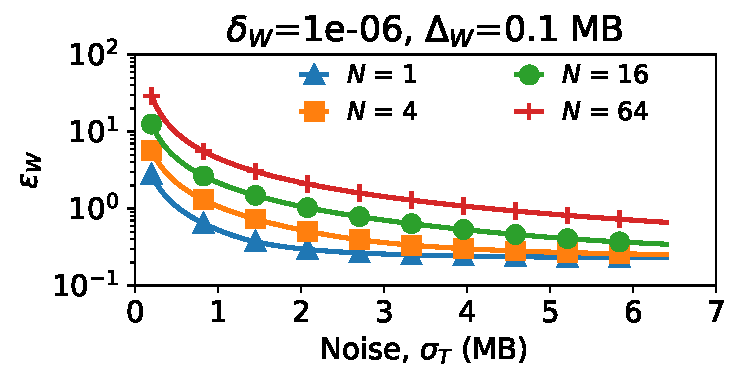
\includegraphics[width=\textwidth]{plots/privacy_loss_VS_noise_std_low_sensitivity.pdf}
      \caption{}
      %        \caption{Noise vs privacy loss}
      \label{subfig:low-sensitivity-epsilon-sigma}
  \end{subfigure}
  \hfill
%    \begin{subfigure}{0.33\textwidth}
  %        \centering
  %
  %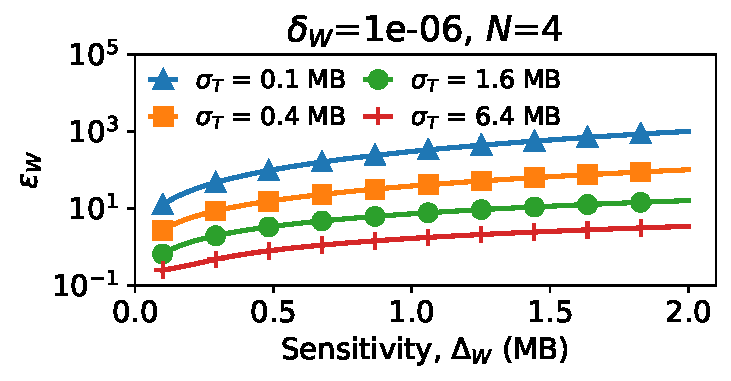
\includegraphics[width=\textwidth]{plots/privacy_loss_VS_sensitivity_video.pdf}
  %        \caption{Sensitivity vs privacy loss}
  %        \label{subfig:high-sensitivity-epsilon-sensitivity}
  %    \end{subfigure}
%    \hfill
  \begin{subfigure}{0.49\columnwidth}
      \centering
      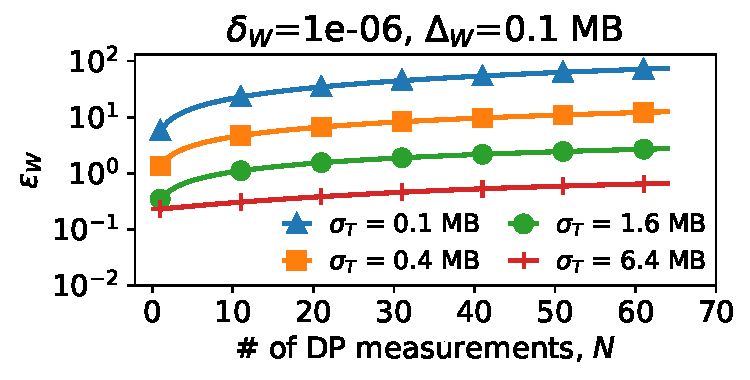
\includegraphics[width=\textwidth]{plots/privacy_loss_VS_query_num_low_sensitivity.pdf}
      \caption{}
%        \caption{\# of DP measurements vs privacy loss}
      \label{subfig:low-sensitivity-epsilon-queries}
  \end{subfigure}
  \caption{
    Per-window privacy loss ($\varepsilon_{\winlen}$) as a function of
    (a) noise ($\sigma_\dpintvl$), and (b) number of DP measurements ($N$).
%    \am{Make notations consistent.}
  }
  \label{fig:privacy-microbenchmarks-low-sensitivity}
\end{figure}